\documentclass[norsk]{beamer}
 
\usepackage[T1]{fontenc}
\usepackage{textcomp,pdfpages}
\usepackage{babel}

\usepackage{amsmath, amsfonts, epsfig, xspace}
\usepackage{pstricks,pst-node}
\usepackage{multimedia}
\usepackage{beamerthemesplit}
\usepackage[absolute, overlay]{textpos}

\usetheme{bekk}

\author{Aslak Johannessen \\ aslakjo@bekk.no  @aslakjo}

\title[Appengine]{Google Appengine}
\subtitle[]{Hosting for alle}
\institute{BEKK Consulting AS}


\begin{document}

\maketitle

\kontrast{Aslak Johannessen \\\small aslakjo@bekk.no \\ @aslakjo}

\kontrast{I gamle dager!}

\begin{frame}{Google Appengine}
  \begin{content}
    \begin{textblock}{10}(5,0)
      
\includegraphics[scale=0.3]{google}\\
      
\includegraphics[scale=0.5]{gae}
    \end{textblock}
    \begin{itemize}
      \item Hosting
      \item Cloud / skyen      
      \item Gratis
    \end{itemize}
  \end{content}
\end{frame}

\kontrast{Ide!}
\kontrast{Hacking!}
\kontrast{?}

\begin{frame}{Hosting}
  \begin{content}
    \begin{itemize}
      \item Noen m� kj�re webappen din
        \subitem{Hosting}
      \item Den m� v�re der
        \subitem{Oppetid}
      \item Billig / gratis
        \subitem{Pris}
      \item Enkelt
        \subitem{Deployment}
    \end{itemize}
  \end{content}
\end{frame}


\begin{frame}{Cloud / skyen}
  \begin{content}
    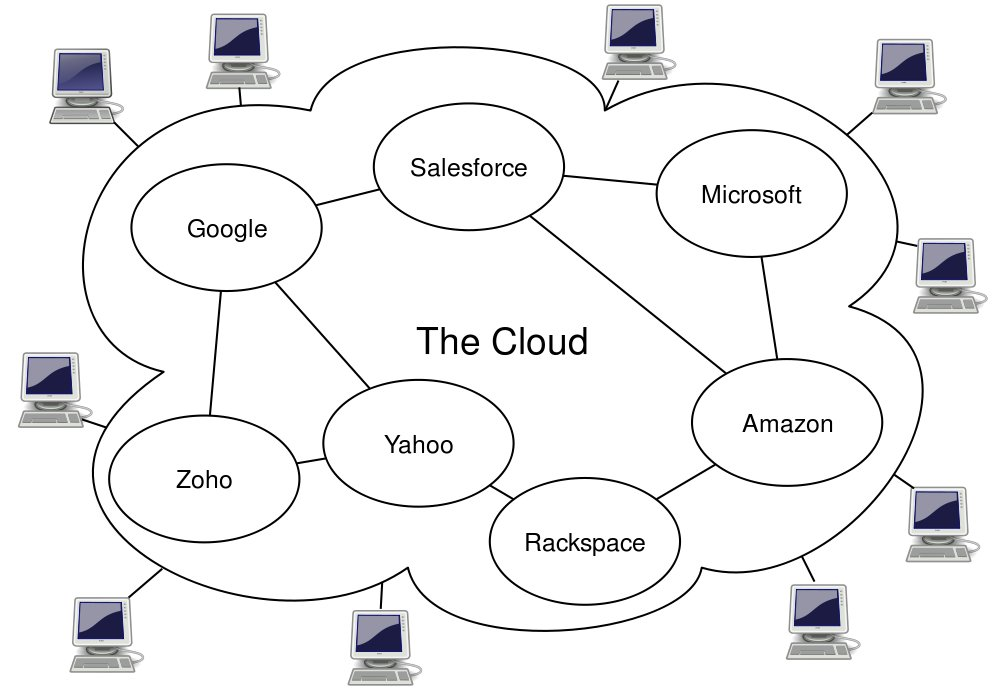
\includegraphics[scale=0.3]{Cloud}
  \end{content}
  \footnote{ Sam Johnston - http://en.wikipedia.org/wiki/File:Clou\_computing.svg }
\end{frame}

\begin{frame}{Cloud / skyen}
  \begin{content}
    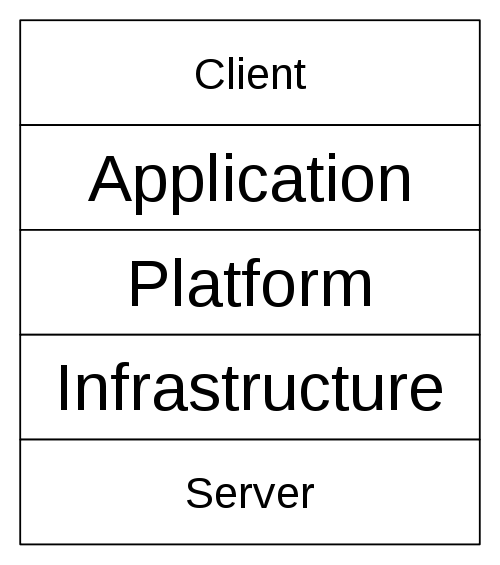
\includegraphics[scale=0.3]{cloud-stack}
  \end{content}
  \footnote{ http://en.wikipedia.org/wiki/File:Cloud\_Computing\_Stack.svg }
\end{frame}

\begin{frame}{Andre}
  \begin{content}
    
\includegraphics[scale=0.3]{heroku}
    
\includegraphics[scale=0.3]{azure}
    
\includegraphics[scale=0.3]{amazon}\\
    
\includegraphics[scale=0.3]{playapps}
    
\includegraphics[scale=0.3]{spotify}
    
\includegraphics[scale=0.3]{dropbox}
  \end{content}
\end{frame}

\begin{frame}{Gratis}
  \begin{content}
    \begin{itemize}
      \item Student
        \subitem{Lite med penger}
      \item Ny grynder 
        \subitem{Lite med penger}
      \item Lite komersiell / eksprimentell ide
        \subitem{Lite med penger}
    \end{itemize}
  \end{content}
\end{frame}


\begin{frame}{Gratis - trodde du} 
  \begin{content}
    \begin{itemize}
      \item Betaler for de du bruker
      \item Gratis ved lite bruk
        \subitem{GAE req < 43,200,000, CPU < 6.5 CPU-hours(100\%}
      \item S� for de aller fleste forhold -- Gratis
    \end{itemize}
  \end{content}
\end{frame}

\kontrast{Hvordan!}

\begin{frame}[fragile]{Appserver}
  \begin{content}
  Appengine er en (nesten) standard appserver.\\

  \tiny
  \begin{verbatim}
    /
    /WEB-INF/
    /WEB-INF/appengine-web.xml
    /WEB-INF/web.xml
    /WEB-INF/classes/aslakjo/HelloWorldServlet.class
    /WEB-INF/lib/
  \end{verbatim}

  \begin{verbatim}
     <web-app>
       <servlet>
           <servlet-name>HelloServlet</servlet-name>
           <servlet-class>aslakjo.HelloWorldServlet</servlet-class>
       </servlet>
       <servlet-mapping>
           <servlet-name>HelloServlet</servlet-name>
           <url-pattern>/hello</url-pattern>
       </servlet-mapping>
     </web-app>
  \end{verbatim}
  \end{content}
\end{frame}


\kontrast{
\includegraphics[height=5em]{duke} \\javax.servlet.http.HttpServlet \\ ant package || mvn war:war}

\kontrast{
\includegraphics[height=5em]{ror} \vspace{5pt} 
\includegraphics[height=5em]{rduke}\\Ruby on Rails \\ \$> jruby warbler}

\kontrast{
\includegraphics[height=10em]{gae-java} \\ Demo}

\begin{frame}{Begrensninger}
  \begin{content}
    Appengen er bare \textbf{nesten} en vanlig appserver. 
    \begin{itemize}
      \item Lagring p� Google BigTable
        \subitem{Det finnes l�snninger for JPA, men de funker bare i det sm�.}
      \item Sikkerhetspolicy
        \subitem{Ingen tr�der}
        \subitem{Ikke alle JDK klasser er tilgjennelige}
        \subitem{Egene begrensning p� standard APIet}
        \subitem{Egen classloader}
    \end{itemize}
  \end{content}
\end{frame}

\begin{frame}[plain]
  \begin{centering}
    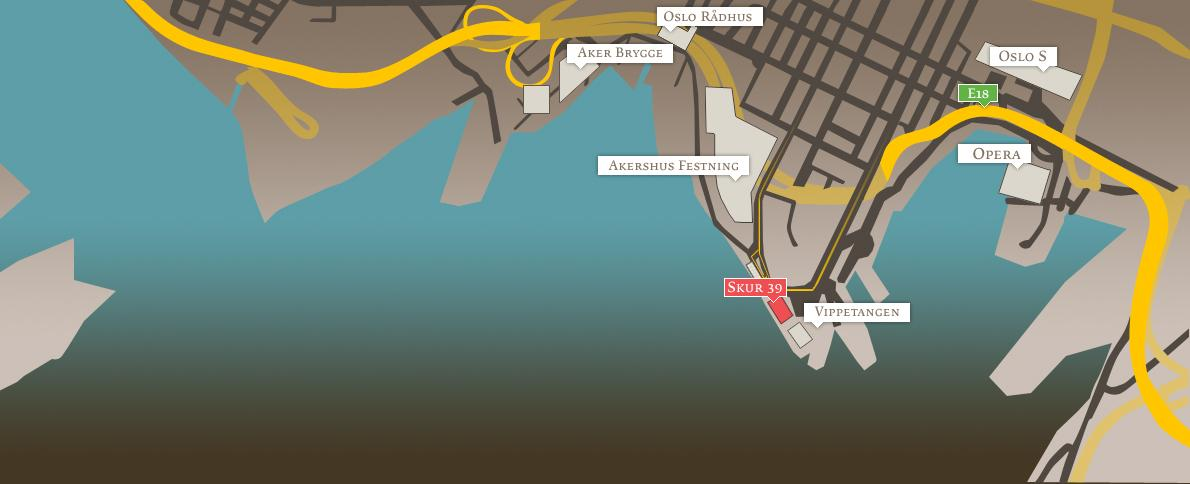
\includegraphics[height=11em]{bekk}
    \\\vspace{2em}\hfill\\
    \small
    
\includegraphics[height=1em]{bekk-logo}
    \\\vspace{.4em}\hfill\\
    \fontsize{8}{8}
\kontrast{
\includegraphics[height=5em]{ror} \vspace{5pt} 
\includegraphics[height=5em]{rduke}\\Ruby on Rails \\ \$> jruby warbler}
    \selectfont
    \textbf{Aslak Johannessen}\\
    Senior Consultant\\
    982 19 249 \\
    aslakjo@bekk.no\\
    \vspace{.3em}\hfill\\
    \fontsize{1}{1}
    \selectfont
    BEKK CONSULTING AS\\
SKUR 39, VIPPETANGEN. P.O. BOX 134 SENTRUM, 0102 OSLO, NORWAY. WWW.BEKK.NO\\


  \end{centering}
\end{frame}

\end{document}
